\section{AWARE}\label{sec:aware}

The purpose of the Automated Wave Analysis and Reduction in EUV (AWARE) algorithm (see Fig. 3) is to detect and characterize the fundamental properties of EUV waves, and make those detections available to the solar community. Automated feature detection algorithms have an advantage over human detections of features because they generate repeatable results for the same input data. AWARE is written in Python and makes use of features provided by the SunPy data analysis package.

%\begin{figure}
%\begin{center}
%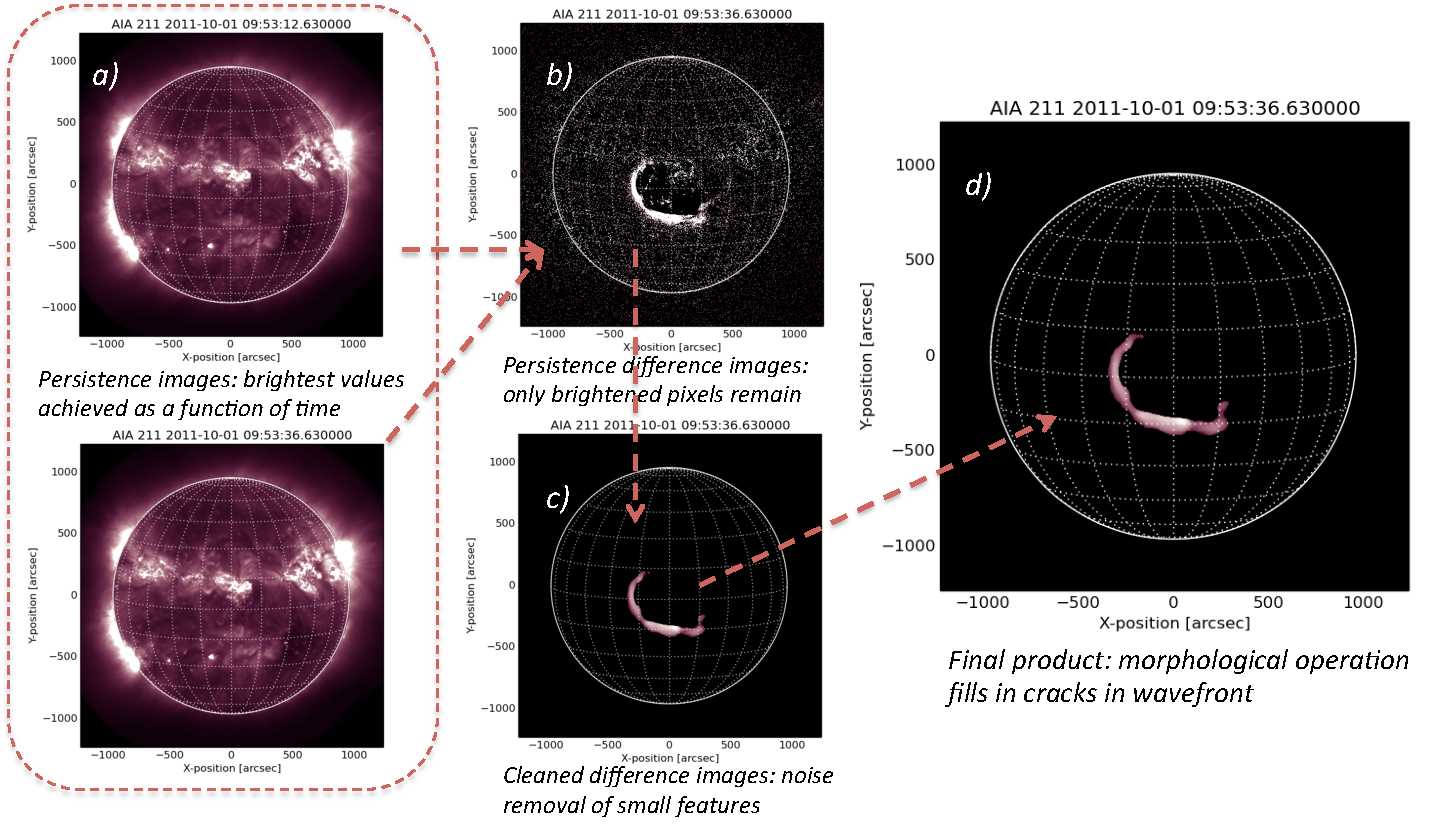
\includegraphics[width=16cm]{aware_figure4.pdf}
%\caption{Caption here}
%\end{center}
%\end{figure}

\subsection{Data Acquisition}


\subsection{Image Processing}

As was noted in Sections 1 and 2, EUV waves are difficult to detect since they are faint, extensive and propagate over a complex background image (the solar corona).  We have recently developed a new, simple and very promising strategy for segmenting an EUV wave wavefront from image data.  The image processing steps for this strategy are given below, and examples of the application of these steps are shown in Fig. 4.

\begin{itemize}
\item Create persistence images of the image data.  A persistence image is found by calculating the persistence value of a pixel at all locations and times \citep[e.g.][]{2014AAS...22421838T}.  The persistence value is simply the maximum value reached by that pixel in the time range 0→t.  If at later times the pixel value increases, the persistence value increases accordingly. If the pixel value decreases however, the persistence value remains unchanged. A persistence movie indicates the brightest values yet achieved in an image sequence.  Brightness can only increase in movies of persistence images (Fig. 4a). 


\item Take the running difference of the persistence images. Only areas that increase in brightness from one time to the next remain (Fig. 4b).

\item Apply a noise reduction filter (Fig. 4c).  Our demonstration algorithm uses a simple two step process.  Firstly, all pixel values below a certain threshold are set to zero.  Secondly, a median filter with scale size L=11 pixels is applied.  This replaces every pixel in the image with the median value found in its neighborhood, a disk of radius 11 pixels.

\item Apply a morphological closing \citep{2002dip..book.....G} operation to every frame in the movie (a disk with radius 11 pixels).  This operation helps close small ‘cracks’ in structures \citep{2002dip..book.....G}.  The final image is shown in Fig. 4d.
\end{itemize}

The final product is therefore a time-ordered series of images that localize the bright wavefront of the EUV wave.

%\begin{figure}
%\begin{center}
%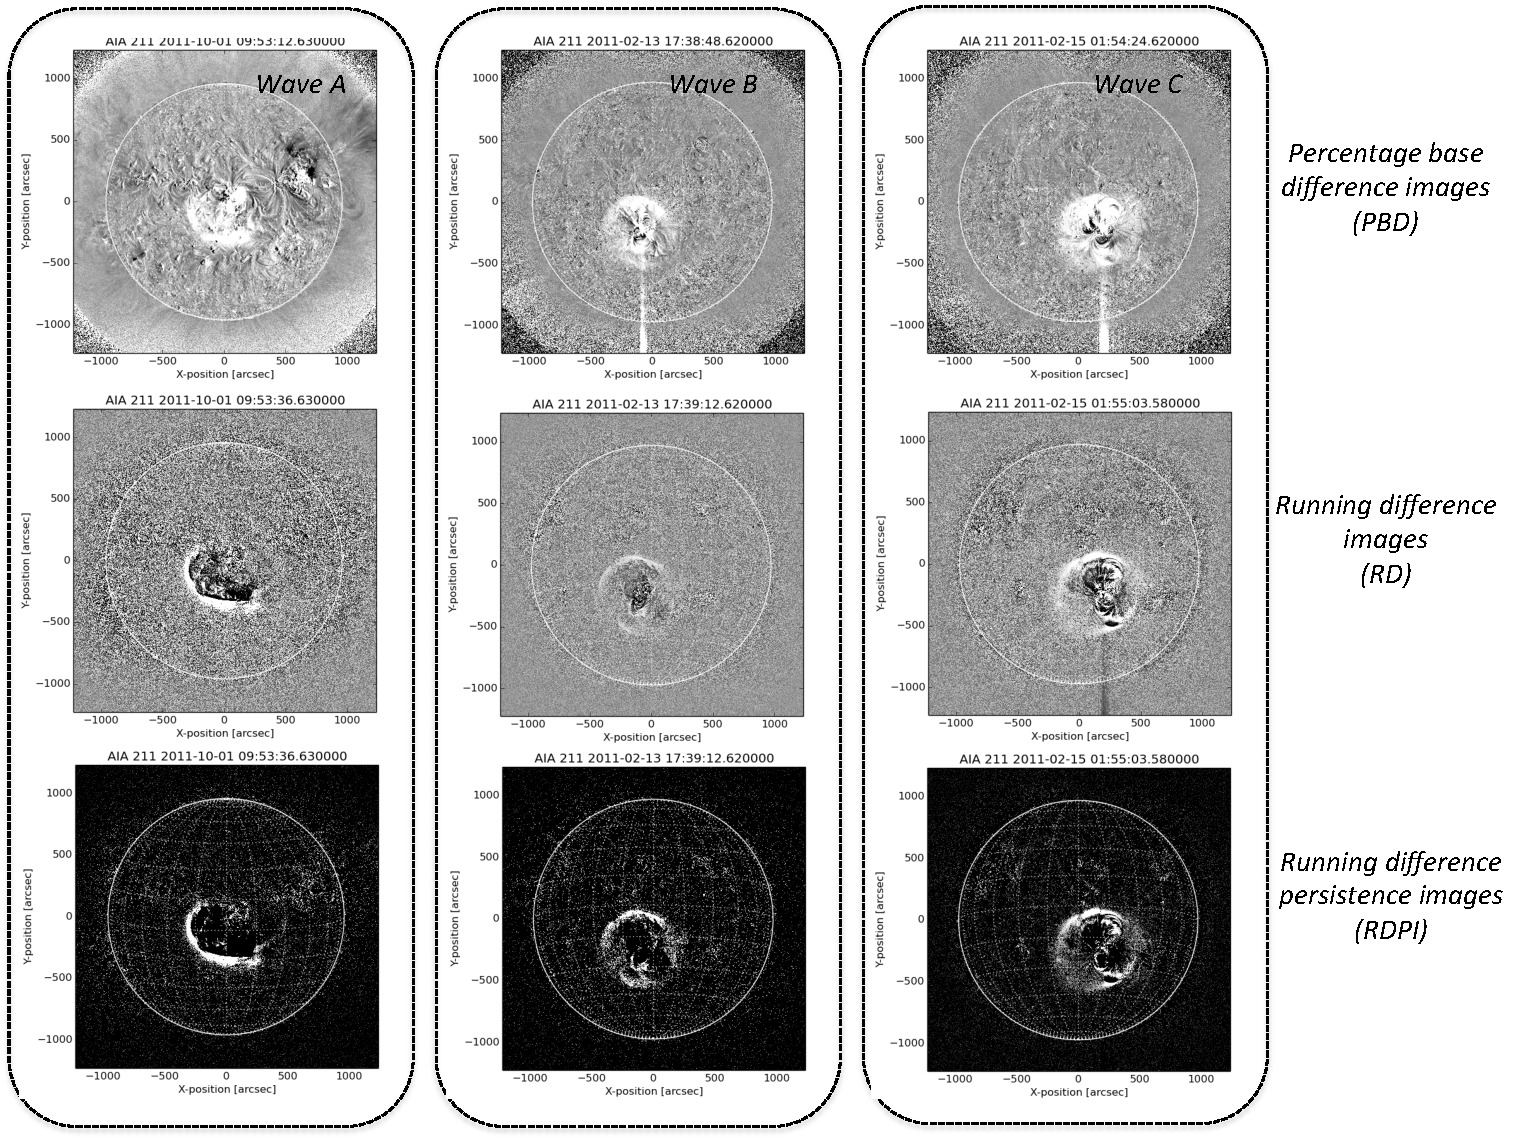
\includegraphics[width=16cm]{aware_rdpm_figure_v3.pdf}
%\caption{Caption here}
%\end{center}
%\end{figure}



Figure 4 shows that the key step is the creation of running differences of time-ordered persistence images (Fig. 4b, see also Fig. 2, bottom row).  Only pixels that brighten over previous values have a non-zero value in the running difference of persistence images.  Zero-value pixels correspond to areas that did not increase in brightness.  Running difference persistence images (RDPIs) have two desirable properties when searching for EUV waves.  Firstly, since an EUV wave brightens neighboring pixels as it moves across the Sun, the RDPIs isolate those brightening pixels.  In other words, the RDPIs isolate the leading part of the wavefront that brightened new pixels.  Secondly, since much of the corona does not vary significantly during an EUV wave, RDPIs show very little residual coronal structure distant from the EUV, greatly simplifying the resulting images.  

The advantages of RDPIs over other common initial steps of isolating propagating features are shown in Fig. 2 for three example EUV wave events. Waves B and C from Fig. 2 were also analyzed by CorPITA in the demonstration of that algorithm by \citet{2014SoPh..289.3279L}.  The first row shows PDB images of each event, the basic image type analyzed by the CorPITA algorithm.  The second row shows RD images, the basic image type analyzed by the NEMO algorithm.  The third row shows RDPI images, the basic image type analyzed by AWARE. Comparison with RDPIs (Fig. 2, bottom row) shows that in standard RD or PBD images the wavefront is more diffuse, and much coronal structure not associated with the wavefront remains in the image. RD and PBD images also have much denser noise compared to the RDPIs of the same data; hence, separating the EUV wave from the noise is substantially easier when using RDPIs.   

Steps 3 and 4 of the AWARE image processing method (Fig. 4c, 4d) apply some basic noise reduction and feature enhancement techniques to further refine the final images.  The bulk of the development phase of AWARE will consist of exploring image processing techniques for noise reduction, feature enhancement and feature segmentation in order to maximize the information about the wavefront \citep[see][ch. 3, 4, 5, 9 \& 10 for many potential improvements]{2002dip..book.....G}.  For example, we will test the efficacy of making the noise threshold in Step 3 time-dependent, to account for the weakening of the wavefront as it propagates.  In Step 4, we will apply the morphological closing operation using multiple length-scales, and average those results: this will test if a multi-scale approach determines more detail in the wavefront.

%\begin{figure}
%\begin{center}
%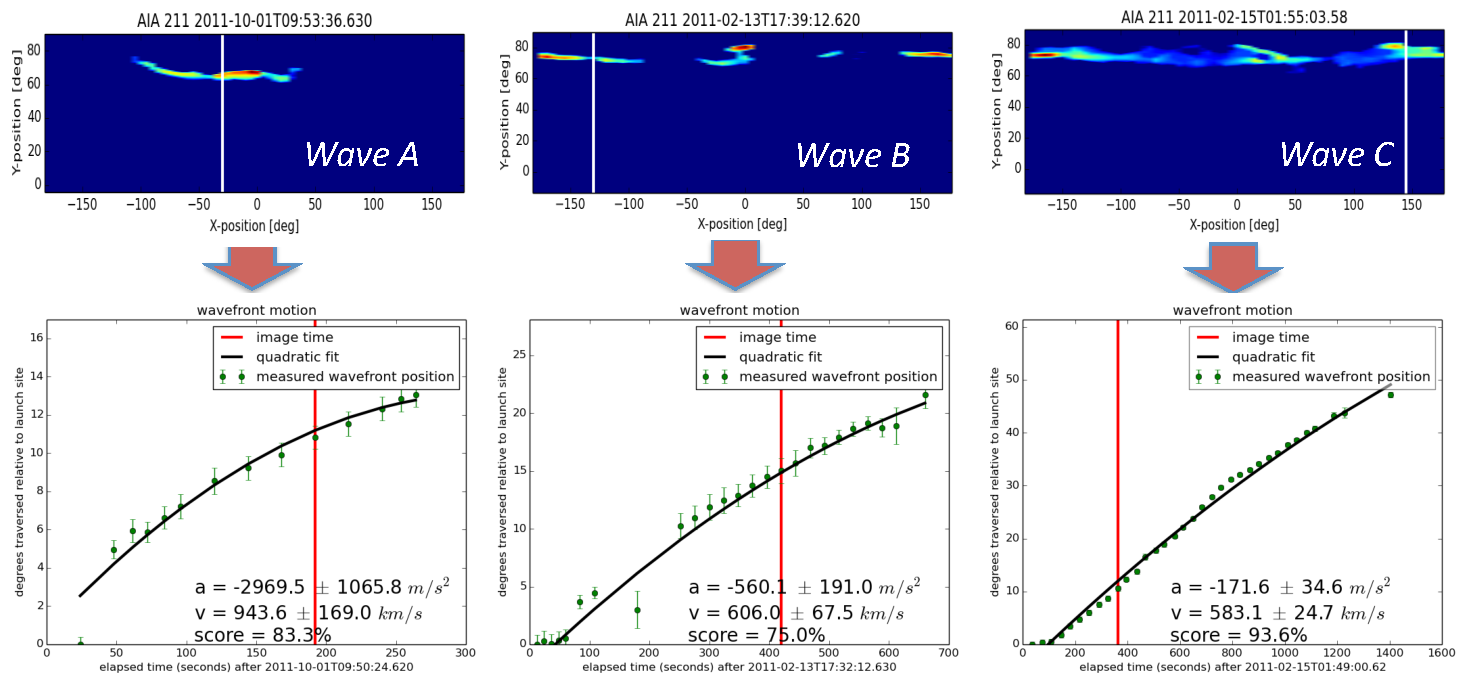
\includegraphics[width=16cm]{aware_velocity_figure_v3.pdf}
%\caption{Caption here}
%\end{center}
%\end{figure}

The advantage of this approach is twofold. Firstly, we do not have to fit a complex profile to noisy data in order to locate the wavefront. Secondly, the RDPIs remove much more structure that is not associated with a propagating bright front (Fig. 2, bottom row) compared to the PBD images (Fig. 2, top-row), and therefore better isolates the wavefront, making noise-cleaning easier (Fig. 4).  NEMO \citep{2005SoPh..228..265P} uses integrals of annuli of RD images (Fig. 2, middle row) to make their detections (Sec. 2.3).  The advantage of our approach over NEMO is also twofold.  Firstly, some EUV waves do not propagate circularly (for example, wave A, Fig. 2) and therefore the annular assumption can lead to a weakened detection.  Secondly, RD images contain dimming and brightening structure unconnected with the EUV wavefront, and are noisier,  when compared to RDPIs, making isolation of the wavefront from these confounding features more difficult. The final result of the first component of AWARE is a time-series of images that may contain an EUV wave.  The second component of AWARE detects the presence of a wave, assesses its quality, and characterizes its propagation through the solar atmosphere.
